\section{Workflow} % (fold)
\label{sec:workflow}
	Im folgenden Abschnitt soll erläutert werden, wie ein moderner Workflow aussehen kann. Dabei sollen viele Aufgaben die oft noch per Hand erfolgen, automatisiert werden.\\

	\subsection{Nodejs \& Node Package Manager} % (fold)
	\label{sub:node_package_manager}
		Nodejs ist eine auf Google Chromes Javascript Runtime aufbauende Plattform und ist unter \url{http://nodejs.org} kostenlos zu bekommen. Nodejs liefert einen eigenen Paket Manager namens "`Node Package Manager"' kurz: "`npm"'.\\

		Npm erlaubt das Installieren von Paketen. Ein Paket ist ein Programm, ein Framework (wie zum Beispiel Bootstrap) oder kann eine beliebige andere Art von Ressource sein, die über die npm-Umgebung zur Verfügung gestellt wird. Pakete können sowohl Global auf dem eigenen Rechner, als auch nur für ein bestimmtes Projekt installiert werden. Der Vorteil von einem Paket Manager wie npm liegt in der Zeitersparnis. Es lassen sich diese Pakete direkt per Befehl in die Kommandozeile eingeben. Dadurch spart man sich das Aufrufen der Webseite im Browser, als auch das Suchen, Herunterladen und Entpacken der gewünschten Datei.\\

		Ein Beispiel: Das Paket "`tmi - too many images"' ist ein kleines Programm, dass eine gegebene URL nach ihrer totalen Bildgröße analysiert und diese mit der durchschnittlichen Größe des Webs vergleicht. Es lässt sich mittels \texttt{npm}-Befehl über die Kommandozeile installieren. Danach lässt es sich ganz einfach per Befehl aufrufen:
		\begin{figure}[htbp]
			\begin{center}
				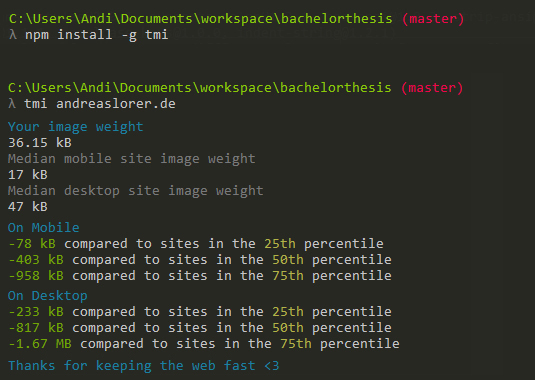
\includegraphics[width=0.7\textwidth]{npm_install_tmi.jpg}
				\label{fig:npm_install_tmi}
			\end{center}
		\end{figure}
		

		Es wäre aber auch möglich das unter Punkt \ref{ssub:google_pagespeed_insight} vorgestellte \texttt{Google Pagespeed Insight}, mittels "`npm install -g psi"' (-g steht für: Global) zu installieren und per "`psi someURL.de"' aufzurufen. Es gibt bereits mehr als 134,082 Pakete (Stand 21.03.2015), die verschiedenste Aufgaben erledigen können. Das Spektrum an Paketen ist sehr groß und reicht von sinnlosen Aufgaben (wie dem zufälligen generieren von Katzennamen\footnote{Cat-names: \url{https://www.npmjs.com/package/cat-names}}) bis hin zu hoch komplexen Programmen wie "`sitespeed.io"'\footnote{Sitespeed.io: \url{http://www.sitespeed.io/}}, das eine rekursive Performance-Analyse einer ganzen Webanwendung ermöglicht.\\

		\subsubsection{Dependency Management} % (fold)
		\label{ssub:dependency_management}
			Dependendcy Management bedeutet, dass ein Projekt oftmals auch noch von anderen Ressourcen abhängt. Das kann eine Library oder ein Framework wie Bootstrap sein. Dieses Framework seinerseits kann seinerseits wieder von externen Ressourcen abhängen. Im Falle von Bootstrap hängt dieses von JQuery ab. 
			Der klassische Weg, wie solche externe Abhängigkeiten im Projekt geregelt werden, sieht wie folgt aus:
			\begin{itemize}
				\item Zu Beginn des Projekts werden Bibliotheken und Frameworks heruntergeladen.
				\item Es folgt das Entpacken und das Verschieben in das richtige Projektverzeichnis.
				\item Erscheint beispielsweise eine neue Version des Frameworks, beginnt dieser Prozess von neuem.
			\end{itemize}

			Dependency Manager (wie z.B. npm oder Bower) schaffen hier Abhilfe und vereinfachen diese Schritte. Durch Ausführen des Befehls: "`npm init"' lässt sich eine neue Abhängigkeitsstruktur für ein Projekt anlegen. Dabei wird eine Datei mit dem Namen: "`package.json"' und ein Ordner mit dem Namen "`node\_modules"' erzeugt. In dieser Datei werden nun sowohl die Beschreibung, die Version, als auch alle Abhängigkeiten gespeichert. Will man nun beispielsweise "`JQuery"' installieren, erfolgt das ganz einfach über das Kommando:
			\begin{lstlisting}[captionpos=b, caption=, label=lst:npm-install]
			npm install -save jquery
			\end{lstlisting}
				
			Die \texttt{-save} Option gibt die Anweisung, dass folgender Eintrag in die package.json Datei aufgenommen werden soll:

			\begin{lstlisting}[captionpos=b, caption=, label=lst:dependencies]
			{
			  "dependencies": {
			    "jquery": "^2.1.3"
			  }
			}
			\end{lstlisting}

			\texttt{\textasciicircum 2.1.3} bedeutet dabei, dass für dieses Projekt mindestens eine JQuery Version größer als 2.1.3 vorliegen muss. Der große Vorteil besteht nicht nun darin, dass weder ein Seitenaufruf getätigt, noch die Dateien entpackt und verschoben werden müssen. Zudem lassen sich über den Befehl "`npm update"' alle Pakete auf die neuste Version bringen, ohne das der Vorgang des erneuten Herunterladen und Entpacken wiederholt werden muss. Die package.json Datei sollte in die Versionskontrolle des Projekts hinzugefügt werden. Der von npm angelegte Ordner: "`node\_modules"' sollte dabei unbedingt per \texttt{.gitignore} von der Versionierung ausgeschlossen werden. Lädt ein Teammitglied das Repository herunter, so muss nur noch "`npm install"' aufgerufen werden und alle Abhängigkeiten, mit den für dieses Projekt verwendeten Versionsnummern, werden automatisch heruntergeladen und installiert. Damit ist jedes Teammitglied auf dem selben Stand und verwendet die selben Versionen. Neue Abhängigkeiten lassen sich so auch ganz einfach an alle Mitglieder verteilen.
			
		% subsubsection dependency_management (end)

		\subsubsection{Bower} % (fold)
		\label{ssub:bower}
			Wie \texttt{npm}, so ist auch \texttt{Bower} ein Paket Manager. Um genau zu sein basiert Bower auf npm und lässt sich mittels "`npm install -save bower"' für das Projekt installieren. Der Vorteil von Bower besteht darin, dass über eine \texttt{.bowerrc} Datei angeben werden kann, in welchem Ordner die Pakete installiert werden sollen. Dies ist bei npm nicht möglich.\\
			Es lohnt sich Frameworks und Libraries wie z.B. \texttt{Bootstrap} oder \texttt{Underscore} mittels Bower zu installieren und andere Programme, wie zum Beispiel Gulp oder andere Nodejs Module, per npm.\\
			Bower lässt sich, ähnlich wie npm, über das Kommando: "`bower init"' Initialisieren. Danach lassen sich per Befehl "`bower install -save bootstrap"' das Bootstrap Framework installieren. 

			\begin{figure}[htbp]
				\begin{center}
					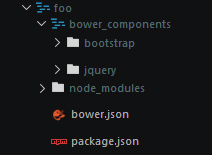
\includegraphics[width=0.35\textwidth]{bower_structure.jpg}
					\caption{Projektstruktur mit npm und Bower}
					\label{fig:bower_structure}
				\end{center}
			\end{figure}
			
			Wie in Abbildung \ref{fig:bower_structure} zu sehen ist, wurde nicht nur Bootstrap, sondern auch JQuery von Bower installiert. Das liegt daran, dass Bootstrap als interne Abhängigkeit wiederrum auch Abhängigkeiten besitzt. Diese werden bei der Installation von Bootstrap gleich mit installiert. Entfernt man Bootstrap wieder, so würde auch JQuery entfernt werden. Würde Bootstrap in einer neuen Version erscheinen, die von einer höheren JQuery Version abhängt, so würde Bower automatisch auch JQuery auf die nötige Version aktualisieren.
		
		% subsubsection bower (end)

	\pagebreak
	% subsection node_package_manager (end)

	\subsection{Gulp Task Manager} % (fold)
	\label{sub:gulp_task_manager}
		Warum und für was braucht es überhaupt einen Task Manager?
		\begin{quote}
			\textit{If you aren't using productivity tools or task automation, you are working \textbf{too hard.} [...] Automation isn't about being lazy. It's about being \textbf{efficient}.}\autocite[p. 18,78]{addyOsmani14}
		\end{quote}
		Ein Task Manager übernimmt immer wiederkehrende Arbeiten. Dazu zählt zum Beispiel die Aufgabe "`minify, uglify und concatenating"' wie in Punkte: \ref{ssub:ressourcen_reduzieren} bereits beschrieben. Aber auch das Übersetzen von "`Sass"'\footnote{Sass is the most mature, stable, and powerful professional grade CSS extension language in the world. \url{http://sass-lang.com}}, oder das Optimieren und Verkleinern von Bildern lässt sich als Task beschreiben und automatisieren.
		Die zwei bekanntesten Task Manager heißen \texttt{Gulp} und \texttt{Grunt}. Hier soll das Arbeiten mittels Gulp beschrieben werden, denn er ist sehr viel einfacher zu benutzen als Grunt.

		\begin{figure}[htbp]
			\begin{center}
				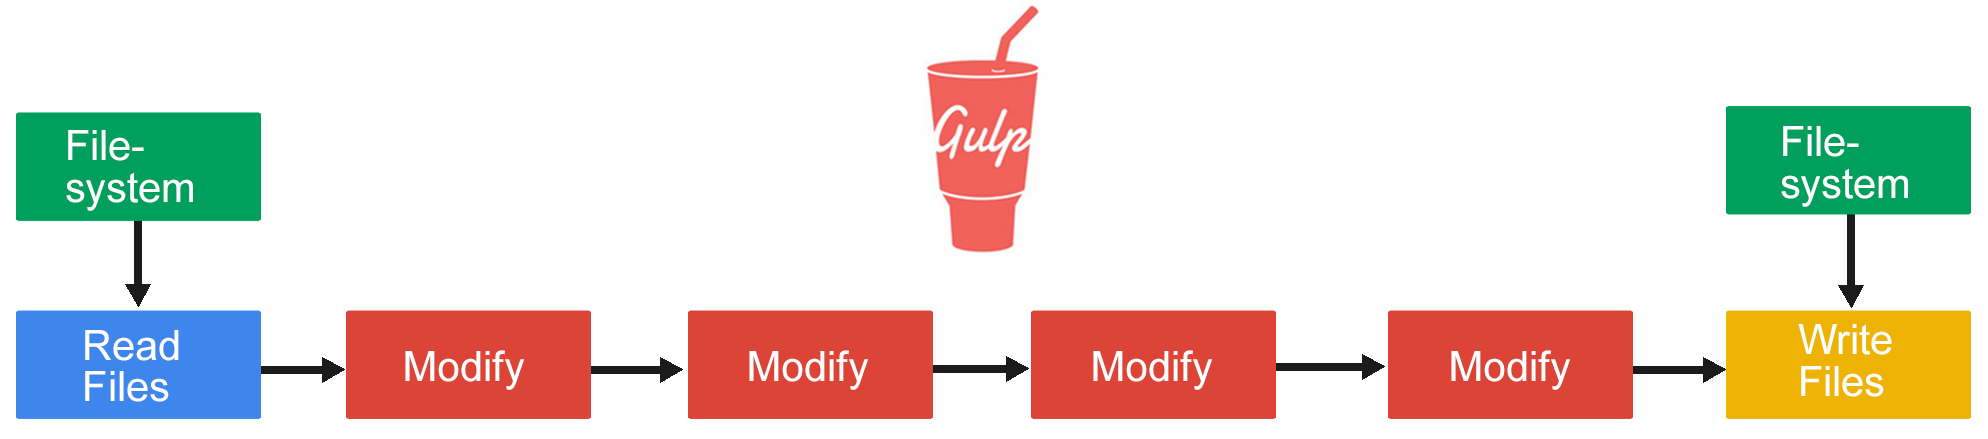
\includegraphics[width=\textwidth]{gulp.jpg}
				\caption{Gulp arbeitet nach dem "`file stream"' Prinzip (Eigene Abbildung nach \autocite[p. 85]{addyOsmani14})}
				\label{fig:gulp}
			\end{center}
		\end{figure}

		Gulp besteht nur aus 4 Kommandos:
		\begin{enumerate}
			\item gulp.task: Definiert einen Namen für einen Gulp Task. Dadurch wird dieser Task über die Kommandozeile benutzbar. Für Anwender, die wenig mit der Kommandozeile arbeiten wollen, gibt es auch eine Google Chrome Browsererweiterung namens Gulp-devtools. Damit lassen sich die verschiedenen Tasks ganz einfach über eine Benutzeroberfläche anklicken.

			\item gulp.src: Greift auf eine oder mehrere Dateien zu. Auch Ordner können angegeben werden.

			\item gulp.dest: Schreibt die Datei in den angegebenen Ort. Durch die Verwendung des *-Zeichens, lässt sich eine \texttt{Wildcard}\footnote{Wildcard bezeichnet im Computer-Bereich einen Platzhalter für andere Zeichen} vergeben. Mittels "`images/*.jpg"' lassen sich zum Beispiel alle jpg-Dateien aus dem Ordner "`images"' auswählen.

			\item pipe: Mittels "`pipe"' lassen sich die Dateien (auch "`file streams"'  genannt) modifizieren. Dabei lässt sich pipe beliebig oft aufrufen. Die Aufgabe: "`minify, uglify und concatenating"' könnte dabei so erfolgen:

		\end{enumerate}

		\begin{lstlisting}[captionpos=b, caption=, label=lst:]
		// require the gulp modules needed:
		var gulp = require('gulp');
		var uglify = require('gulp-uglify');
		var concat = require('gulp-concat');

		// javascript task: concat, minify, uglify all javascript files in folder:
		gulp.task('javascript', function () {
		    gulp.src(['site/assets/libs/*.js', 'site/assets/js/*.js'])
		      .pipe(concat('bundle.min.js')) 
		      .pipe(uglify())
		      .pipe(gulp.dest('dist/assets/js/'));
		});
		\end{lstlisting}
		Dieser Task mit dem Namen "`javascript"' holt nun alle Javascript Dateien aus dem Ordner "`libs"' und "`js"', fügt diese zu einer einzigen Datei zusammen und benennt sie "`bundle.min.js"'. Danach erfolgt das "`uglify"' (beinhaltet das "`minify"'). Zum Schluss wird die Datei in den Ordner "`dist/assets/js"' geschrieben. Die Ausgangsdateien werden dabei nicht modifiziert. Es sind auch so genannte "`watch"' Tasks möglich, die bei einer Dateiänderung ausgeführt werden können. So kann der Browser immer dann neu geladen werden, wenn sich eine CSS Datei geändert hat. Dadurch wird ein manuelles neu Laden, um Änderungen zu betrachten, hinfällig.\\	

		Grunt hat gegenüber Gulp den Vorteil, dass es älter ist als sein Konkurrent. Dadurch gibt es viele Pakete, die nur mittels Grunt zur Verfügung stehen. Beispielsweise das Paket "`grunt-responsive-images"'. Damit lassen sich aus einem gegebenen Bild automatisch verschiedenste Bildgrößen herausrechnen und abspeichern. Dies ist besonders hilfreich, wenn man "`responsive images"' wie in Punkt: \ref{ssub:responsive_images} beschrieben, verwenden möchte. Einen Blick auf Grunt kann sich also durchaus lohnen.\\
		
	\pagebreak
	% subsection gulp_task_manager (end)

	\subsection{Yeoman} % (fold)
	\label{sub:yeoman}
		Ein Projekt wird oftmals manuell oder mittels eines Programms, wie zum Beispiel PHP-Storm oder Visual Studio erstellt. Es wird ein passender Projekttyp gewählt und das Programm erzeugt dann eine fertige Ordnerstruktur mit den wichtigsten Dateien. Zum Beispiel so:

		\begin{figure}[htbp]
			\begin{center}
				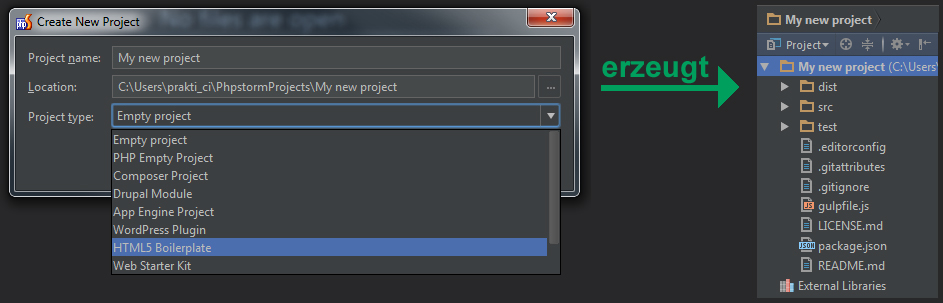
\includegraphics[width=0.9\textwidth]{php_storm_scaffolding.jpg}
				\caption{Projekt erstellen via Php-Storm (Eigene Abbildung)}
				\label{fig:php_storm_scaffolding}
			\end{center}
		\end{figure}
		
		\url{http://yeoman.io/} ist ein Tool für das schnelle Erstellen eines Grundgerüsts für ein Projekt.

		\begin{quote}
			\textit{"`Yeoman helps you to kickstart new projects, prescribing best practices and tools to help you stay productive.\\
			To do so, we provide a generator ecosystem. A generator is basically a plugin that can be run with the `yo` command to scaffold complete projects or useful parts.\\
			Through our official Generators, we promote the "`Yeoman workflow"'. [...] We take care of providing everything needed to get started without any of the normal headaches associated with a manual setup."'} (\url{http://yeoman.io})
		\end{quote}

		Es stellt sogenannte "`Generators"' zur Verfügung, die genau diese Funktionalität der Projekterstellung abbilden. Dabei wird das Ziel verfolgt "`Best Practices"' für das jeweilige Projekt umzusetzen.
		Der Vorteil von Yeoman besteht darin, dass es eine enorme Vielzahl an Generatoren zur Verfügung stellt. So gibt es Generatoren für die Erstellung von Web-Apps, Chrome Browser Erweiterungen, Wordpress Blogs, Firefox OS Apps und noch tausend\footnote{Eine volle Liste an verfügbaren Generatoren ist hier zu finden: \url{http://yeoman.io/generators/}} weitere. 
		Yeoman steht als \texttt{npm} Paket zur Verfügung und lässt sich mittels "`npm install -g yo"' mit Hilfe der Kommandozeile installieren. Via "`npm install -g generator-someName"' lassen sich dann beliebige Generatoren dazu installieren. Yeoman bringt dabei die zuvor vorgestellten Tools wie Gulp / Grunt und Bower zusammen. Durch das Ausführen wird das gesamte Projekt angelegt:
		
		\begin{itemize}
			\item Es werden alle \texttt{npm} Pakete (Bower, Gulp usw.) die nötig sind automatisch installiert.
			\item Die Ordnersturktur mit einer CSS und Javascript Datei wird angelegt und im HTML Dokument eingebunden.
			\item Nach der Installation stehen die wichtigsten Gulp Tasks zur Verfügung, ohne dass man sie selber schreiben muss.
			\item Durch Gulp besteht zum Beispiel die Möglichkeit, einen Webserver mittels Kommando "`gulp serve"' zu starten.
			\item Es bestehen zusätzliche Funktionalitäten wie das automatische Aktualisieren des Browsers nach einer Änderung zur Verfügung.
			\item Mittels Eingabeaufforderung lässt sich auswählen welche Module (Sass, Bootstrap, Modernizr) enthalten sein sollen und welche nicht.
		\end{itemize}

		Das Ausführen von "`yo gulp-webapp"':
		\begin{figure}[htbp]
			\begin{center}
				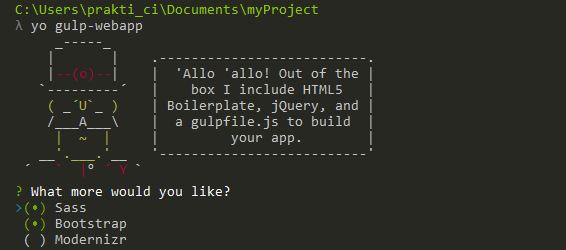
\includegraphics[width=0.7\textwidth]{yeoman_generator.jpg}
				\caption{Starten eines neuen Projekts mittels generator-gulp-webapp (Eigene Abbildung)}
				\label{fig:yeoman_generator}
			\end{center}
		\end{figure}

		würde innerhalb von wenigen Minuten ein Projekt anlegen, das bereits fertig mit Bootstrap, JQuery und einem HTML Dokument konfiguriert ist. Mittels "`gulp serve"' kann das direkt im Browser betrachtet werden:

		\begin{figure}[htbp]
			\begin{center}
				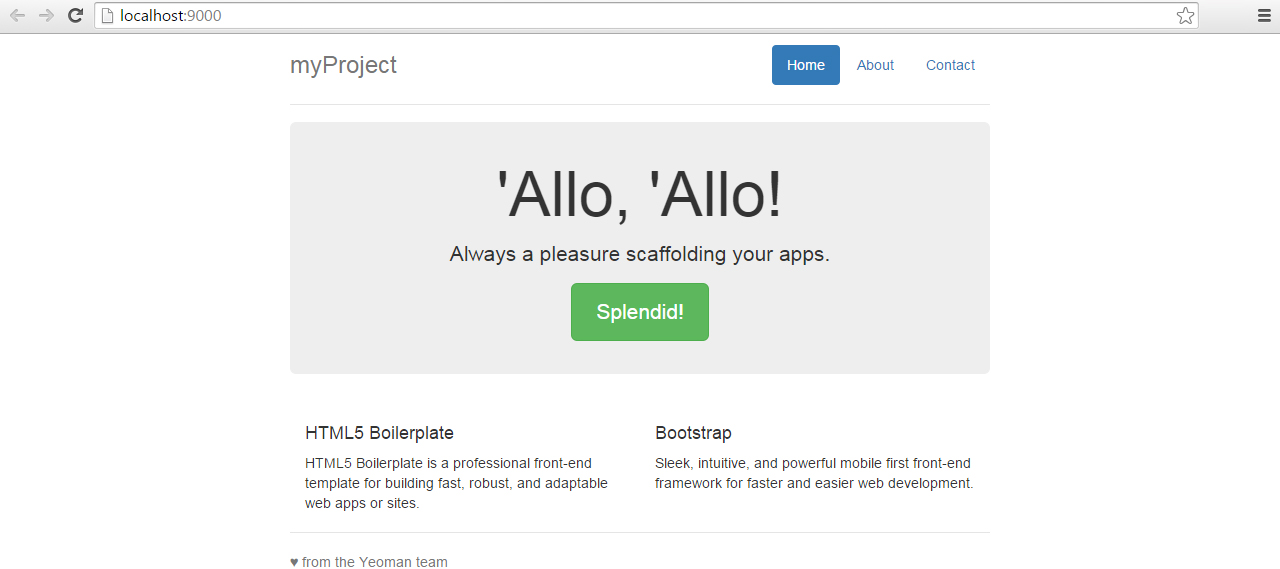
\includegraphics[width=0.8\textwidth]{yeoman_project_start.jpg}
				\caption{Ergebnis des Kommandos: "`yo gulp-webapp"' (Eigene Abbildung)}
				\label{fig:yeoman_project_start}
			\end{center}
		\end{figure}
				
		\subsubsection{Eigene Generatoren erstellen} % (fold)
		\label{ssub:eigene_generatoren_erstellen}
			Yeoman bietet jedem die Möglichkeit, einen eigenen Generator zu erstellen. Auch dafür gibt es wiederrum einen Generator, den "`generator-generator"'. Damit lässt sich eine persönliche Projektstruktur erstellen, die den eigenen Projekten gerecht wird. Dadurch lassen sich beispielsweise Skripte zum verzögerten Laden von Javascript, von Beginn an in das eigene Projekt integrieren. Eigene Generatoren können ganz einfach veröffentlicht werden. Es muss lediglich ein Benutzer mittels "`npm adduser"' angelegt werden und dann kann mittels "`npm publish"' der eigene Generator als \texttt{npm} Paket zur Verfügung gestellt werden. Auch Updates lassen sich mittels "`npm publish"' binnen Sekunden einspielen. Mein persönlicher Generator ist zum Beispiel unter: \url{https://www.npmjs.com/package/generator-4dev} zu finden und kann von jedem über "`npm install -g generator-4dev"' installiert und anschließend mittels "`yo 4dev"' aufgerufen werden.\\

			Für ein Unternehmen könnte dies zum Beispiel bedeuten, mittels einem eigenen Generator eine einheitliche Projektstruktur einzuführen, der die Best Practices des Unternehmens abbildet. Alternativ könnte auch ein Konsens gefunden werden, welcher der bereits existierenden Generatoren für die jeweils eigenen Projekte einzusetzen ist.\\

			Eine ausführliche Anleitung und Dokumentation zur Erstellung von Generatoren ist der offiziellen Seite: \url{http://yeoman.io/authoring/index.html} zu entnehmen.
		
		% subsubsection eigene_generatoren_erstellen (end)
		
	\pagebreak
	% subsection yeoman (end)

	\subsection{Zusammengefasst}
	\label{sub:zusammengefasst}
		Gulp, Bower und Yeoman arbeiten perfekt zusammen und ermöglichen einen modernen Workflow. Mittels \texttt{npm} und \texttt{Bower} lassen sich Pakete ganz einfach installieren, deinstallieren und aktualisieren, während gleichzeitig eine einheitliche Entwicklungsumgebung bereitgestellt wird. Außerdem bieten viele Frameworks die Möglichkeit, mittels Bower, nur einzelne Module zu installieren. Dadurch ist es möglich nur das Nötigste in die Seite einzubinden.\\ Gulp ermöglicht eine umfassende Automatisierung von Aufgaben, die gerade für die Web Performance sehr wichtig sind. Folgende Projektstruktur erweist sich als sinnvoll:

		\lstset{
		 morekeywords={dist,site, node_modules}
		}
		\begin{lstlisting}[captionpos=b, caption=Projektstruktur, label=lst:projectTree]
		.
		|_ site/
		|	|_ bower_components/
		|	|_ index.html
		|	|_ assets/
		|			|_ images/...
		|			|_ js/
		|			|		|_ script_A.js
		|			|		|_ script_B.js
		|			|		|_ script_C.js
		|			|
		|			|_ css/
		|			|		|_ style_A.css
		|			|		|_ style_B.css
		|			|		|_ style_C.css
		|			|_ ...
		|
		|_ dist/
		|		|_ bower_components/
		|		|_ index.html
		|		|_ assets/
		|		|_ images/...
		|		|_ js/
		|		|		|_ script_all.js
		|		|
		|		|_ css/
		|		|		|_ style_all.css
		|		|_ ...
		|
		|_ node_modules/
		|  |_ Gulp
		|  |_ Bower
		|  |_ ..
		|
		|_ gulpfile.js
		|_ package.json
		|_ bower.json
		|_ .gitignore
		|_ ...
		\end{lstlisting}

		"`./site"' ist dabei der Ordner, in dem die Entwicklung stattfindet. Der Ordner "`./dist"' beinhaltet die für die Veröffentlichung angepasste Version von optimierten Bildern, verkleinerte und zusammengefügte CSS und Javascript Dateien und eine Kopie der restlichen, für die Webanwendung wichtigen Elemente. Diese werden automatisch mittels Gulp erzeugt (meistens durch einen sogenannten "`build Task"' ) und lassen sich selbst bei kleinsten Änderungen an der Seite, mit nur einem Kommando neu erstellen. Durch diese Arbeitsweise ist es möglich, dass das Projekt von Beginn an einen für die Veröffentlichung optimalen Stand hat. Gulp bietet für fast alle Aufgaben eine Automatisierung und es lohnt sich ein Blick in die zahllosen Pakete\footnote{Gulp Plugin Suchmaschiene: \url{http://gulpjs.com/plugins/}}, die von einer immer weiter wachsenden Community bereitgestellt werden.\\
		Durch Beachten des kritischen Rendering-Pfads (\ref{sub:critical_render_path}), das Einsetzen der unter Kapitel \ref{sub:tools} vorgestellten Tools und den in dieser Arbeit beschriebenen Optimierungsmaßnahmen, lässt sich eine für den Endanwender akzeptable Ladezeit erreichen.

	% subsection zusammengefasst (end)

% section workflow (end)
\pagebreak